\documentclass[a4paper,11pt]{article}
  
\usepackage{graphicx}
\usepackage{amsmath}
\usepackage{array}
\usepackage{float}
\usepackage{color}
\usepackage{listings}
\usepackage[utf8x]{inputenc}
\usepackage{hyperref}
\usepackage{rotating}
\usepackage[english]{babel}
\usepackage{hyperref}
\usepackage{subfig}
\usepackage{pdfpages}


\usepackage{amsfonts,amsmath,amsthm,amssymb}
\usepackage{algorithm}
\usepackage{algpseudocode}

\renewcommand{\algorithmicrequire}{\textbf{Input:}}
\renewcommand{\algorithmicensure}{\textbf{Output:}}

%% --------- Algorithms -------------
\providecommand{\BeginAlgSize}[0]{\begin{scriptsize}}
\providecommand{\EndAlgSize}[0]{\end{scriptsize}}
\providecommand{\ForEach}[1]{\For{\textbf{each} #1}}
\providecommand{\Or}[0]{O}
\providecommand{\A}[0]{\mathbf{\alpha}}
%% --------- End of Algorithms -------------

% C++ listings settings
\lstset{ %
language=C++,                % choose the language of the code
basicstyle=\scriptsize,       % the size of the fonts that are used for the code
numbers=none,                   % where to put the line-numbers
numberstyle=\footnotesize,      % the size of the fonts that are used for the line-numbers
stepnumber=1,                   % the step between two line-numbers. If it is 1 each line will be numbered
numbersep=5pt,                  % how far the line-numbers are from the code
backgroundcolor=\color{white},  % choose the background color. You must add \usepackage{color}
commentstyle=\color{blue},
showspaces=false,               % show spaces adding particular underscores
showstringspaces=false,         % underline spaces within strings
showtabs=false,                 % show tabs within strings adding particular underscores
frame=single,           % adds a frame around the code
tabsize=2,          % sets default tabsize to 2 spaces
captionpos=b,           % sets the caption-position to bottom
breaklines=true,        % sets automatic line breaking
breakatwhitespace=false,    % sets if automatic breaks should only happen at whitespace
escapeinside={\%*}{*)}          % if you want to add a comment within your code
}

\title{Multiple Vehicle Simulator brief description \\ C++ implemetation in mvsim}
\author{Borys Tymchenko \\ tim4bor@gmail.com}
\date{Document built: \today}

\begin{document}
\maketitle
\vfill
\begin{center}
License: GNU General Public License version 3 Copyright (C) 2017 Jose Luis Blanco jlblanco@ual.es (University of Almeria) and collaborators
\end{center}

\newpage
\tableofcontents
\newpage

\section{Introduction}

The MVSIM is a lightweight, realistic dynamical simulator for 2D ("2.5D") vehicles and robots. It is tailored to analysis of vehicle dynamics, wheel-ground contact forces and accurate simulation of typical robot sensors (e.g. laser scanners).

This package includes the C++ library mvsim, a standalone app and a ROS node.

\newpage

\section{Features}
\begin{itemize}

\item Lightweight in memory, CPU and library requirements.
\item Fully configurable via .xml "world" files.
\item World maps:
	\begin{itemize}	
		\item Occupancy gridmaps: input as images or MRPT binary maps (from icp-slam, rbpf-slam, etc.)
		\item Elevation meshes.
	\end{itemize}	 
\item Vehicle models:
	\begin{itemize}
		\item Differential driven (2 \& 4 wheel drive).
		\item Ackermann steering (kinematic \& dynamic steering, different mechanical drive models).
	\end{itemize}
\item Sensors:
	\begin{itemize}
		\item Laser scanners: Robots see each other, their own bodies, etc.
	\end{itemize} 
\item Interface to vehicles: Choose among:
	\begin{itemize}
		\item Raw access to forces and motor torques.
		\item Twist commands (using internal controllers).
	\end{itemize}

\end{itemize}

\newpage

\section{World simulation}
Simulation happens inside a World object.
This is the central class for usage from user code, running the simulation, loading XML models, managing GUI visualization, etc.
The ROS node acts as a bridge between this class and the ROS subsystem.

World description is loaded using XML files that contain all the information about world.

\subsection{World files}
\textbf{TODO this}
\newpage


\subsection{Simulation execution}
Simulation executes step-by-step with user-defined $\Delta t$ time between steps.
Each step has several sub steps:
\begin{itemize}
\item Before time step - sets actions, updates models, etc.
\item Actual time step - updates dynamics
\item After time step - everything needed to be done with updated state
\end{itemize}

\subsubsection{Logging}

Each vehicle is equipped with parameters logger(s). This logger is not configurable and can be rewritten programmaticaly. 

Logger are implemented via \textbf{CsvLogger} class and make log files in CSV format which then can be opened via any editor or viewer. 

Loggers control is introduced via robot controllers, each controller controls only loggers of its robot. 

Best results in visualizing offers QtiPlot \ref{fig:qtiplot_example1}.

\begin{figure}[h!]%\textsl{}
	\centering
	\subfloat[Velocity vs rolling resistance]{{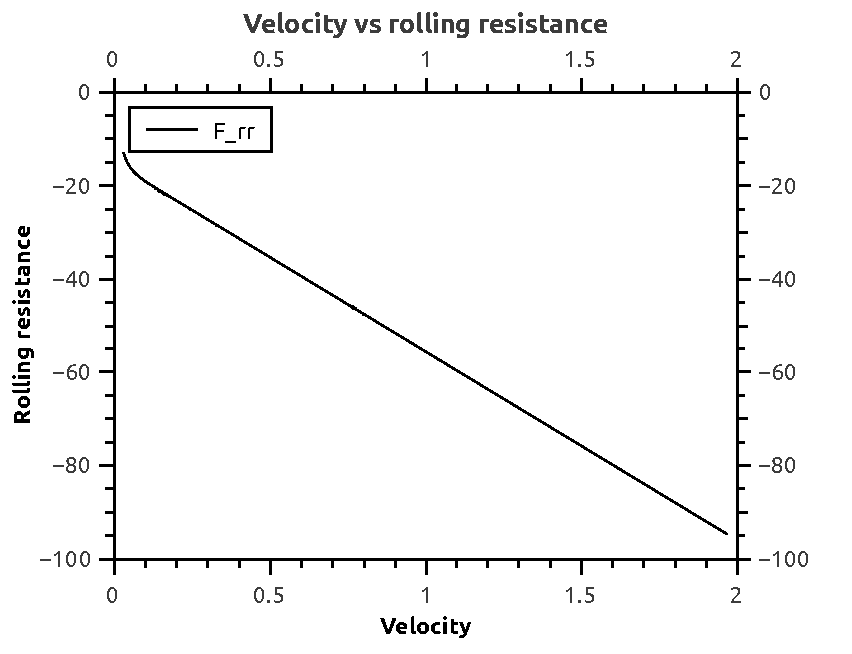
\includegraphics[width=5cm]{imgs/vel_frr} }}%
	\qquad
	\subfloat[Velocity vs drive torque]{{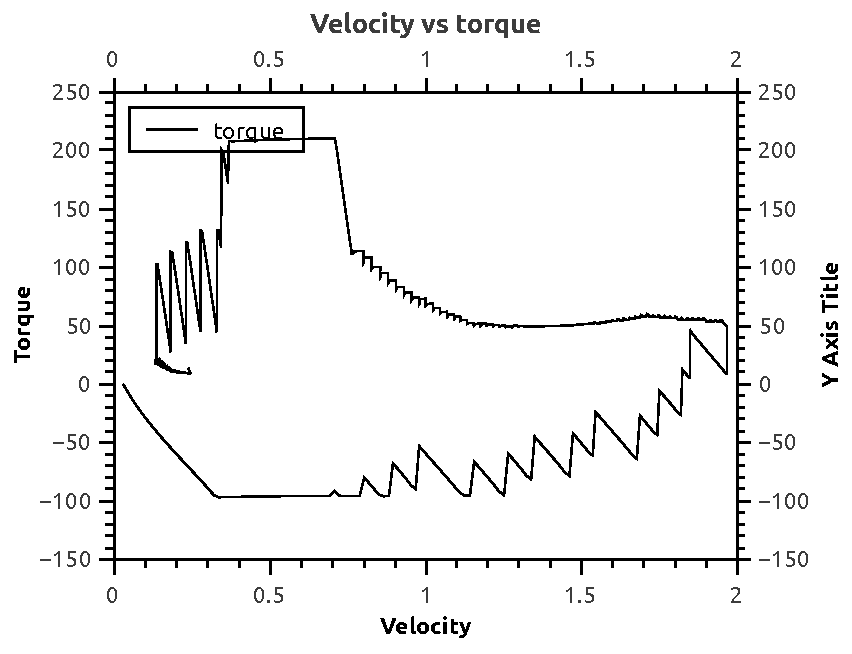
\includegraphics[width=5cm]{imgs/vel_torque} }}%
	\caption{Loggers with QtiPlot example}%
	\label{fig:qtiplot_example1}%
\end{figure}


At the moment, following characteristics are logged: 
\begin{itemize}
	\item Pose ($x, y, z, \alpha, \beta, \gamma$)
	\item Body velocity ($\dot{x}, \dot{z}, \dot{z}$)
	\item Wheel torque ($\tau$)
	\item Wheel weight ($m_{wp}$)
	\item Wheel velocity ($v_x, v_y$)
\end{itemize}

Loggers support runtime clear and creating new session. The new session mode finalizes current log files and starts to write to a new bunch of them.


\newpage

\section{Physics used}
\subsection{Wheel dynamics}

We introduce wheels as a mass with cylindrical shape (Figure \ref{fig:wheel_forces}).
Each wheel has following properties:
\begin{itemize}
\item location of the wheel as to the chassis ref point [m,rad] in local coordinates $L_w = \{ x_w, y_w, \Phi \}$
\item diameter $d_w$ [m]
\item width $w_w$ [m]
\item mass $m_w$ [kg]
\item inertia $I_{yy}$ 
\item spinning angular position $\phi_w$ [rad]
\item spinning angular velocity $\omega_w$ [rad/s]
\end{itemize}

Thus, each wheel is represented as $W = \{L_w, d_w, w_w, m_w, I_{yy}, \phi_w, \omega_w\}$

\begin{figure}[h!]
  \centerline{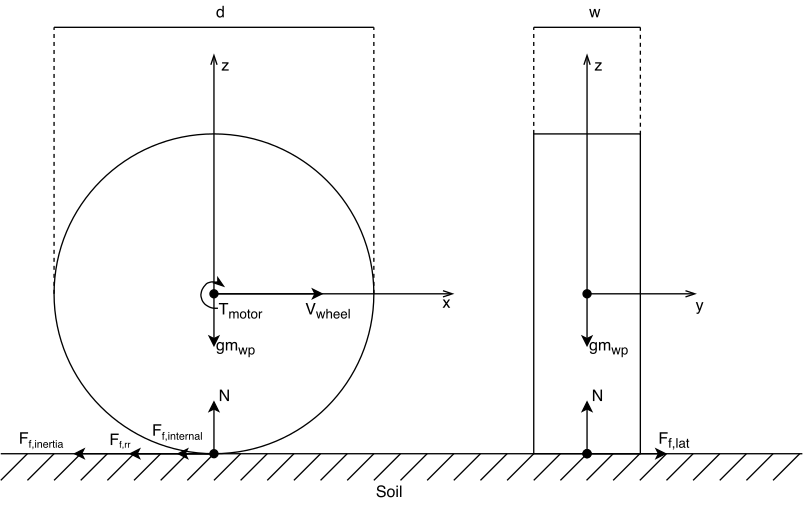
\includegraphics[width=0.7\linewidth]{imgs/wheel_forces}}
  \caption{Wheel forces}
  \label{fig:wheel_forces}
\end{figure}


\subsection{Friction models}
\subsubsection{Friction models base}
Friction model base introduces \textit{Friction input} structure, that incorporates forces of wheel
\begin{itemize}
\item weight on this wheel from the car chassis, excluding the weight of the wheel itself $w$ [N]
\item motor torque $\tau$ [Nm]
\item instantaneous velocity 
\[\nu = \begin{bmatrix}
\nu_x \\
\nu_y
\end{bmatrix}\] in local coordinate frame
\end{itemize}

\subsubsection{Default friction}
At the moment, there is only one basic friction model available for vehicles.
Default friction model evaluates ...

Default friction evaluates forces in the wheel coordinate frame:

\begin{center}
\[
\nu_w = 
\begin{bmatrix}
\nu_{wx} \\
\nu_{wy}
\end{bmatrix}
=R(\Phi_w) \cdot \nu
\]
\end{center}

To calculate maximal allowed friction for the wheel, we introduce partial mass:
\begin{center}
\[
m_{wp} = \frac{w_w}{g} + m_w
\]
\[
F_{f, max} = \mu \cdot m_{wp} \cdot g
\]
\end{center}
Where $\mu$ is friction coefficient for wheel.

Calculating latitudinal friction (decoupled sub-problem):
\begin{center}
\[
F_{f,lat} = m_{wp} \cdot a = m_{wp} \cdot \frac{-\nu_{wy}}{\Delta t}
\]
\[
F_{f,lat} = max(-F_{f,max}, min(F_{f,lat}, F_{f,max}))
\]
\end{center}

Calculating wheel desired angular velocity:

\begin{center}
\[
\omega_{constraint} = \frac{2\nu_{wx}}{d_w}
\]
\[
J_{desired} = \omega_{constraint} - \omega_w
\]
\[
\omega_{desired} = \frac{J_{desired}}{\Delta t}
\]
\end{center}


Calculating longitudinal friction:
\begin{center}
\[
F_{f,lon} = \frac{1}{R} \cdot (\tau - I_{yy}\cdot \omega_{desired} - C_{damp} \cdot \omega_w)
\]
\[
F_{f,lon} = max(-F_{f,max}, min(F_{f,lon}, F_{f,max}))
\]
\end{center}

Simply composing friction forces to vector:
\begin{center}
\[
F_f = 
\begin{bmatrix}
F_{f,lat} \\
F_{f,lon}
\end{bmatrix}
\]
\end{center}

With new friction, we evaluate angular acceleration \textit{(code says angular velocity impulse, but the units are for acceleration)}  of the wheel:
\begin{center}
\[
\alpha = \frac{ \tau - R \cdot F_{f,lon} - C_{damp} \cdot \omega_w}{I_{yy}}
\]
\end{center}

Using given angular acceleration, we update wheel's angular velocity:
\begin{center}
$$
\omega_w = \omega_w + \alpha \cdot \Delta t
$$
\end{center}

\newpage
\subsubsection{Ward-Iagnemma friction}
This type of friction is an implementation of paper from Chris Ward and Karl Iagnemma \cite{ward-iagnemma-friction}.

Rolling resistance is generally modeled as a combination of
static- and velocity-dependant forces [17], [21]. Authors propose function with form similar to Pacejka's model \cite{pacejka_tire_model} as a continuously differentiable
formulation of the rolling resistance with the static force
smoothed at zero velocity to avoid a singularity. The rolling
resistance is


$$
F_{rr} = −sign(V_{fwd}) \cdot N \cdot (R_1 \cdot (1 − e^{−A_{roll} |V_{fwd} |}
)+R_2 \cdot |V_{fwd}|)
$$


Where $A_{roll}$, $R_1$, $R_2$ are the model-dependent coefficients. The impact of these coefficients is shown at figure \ref{fig:wi_rr} taken from original paper.

\begin{figure}[h!]
	\centerline{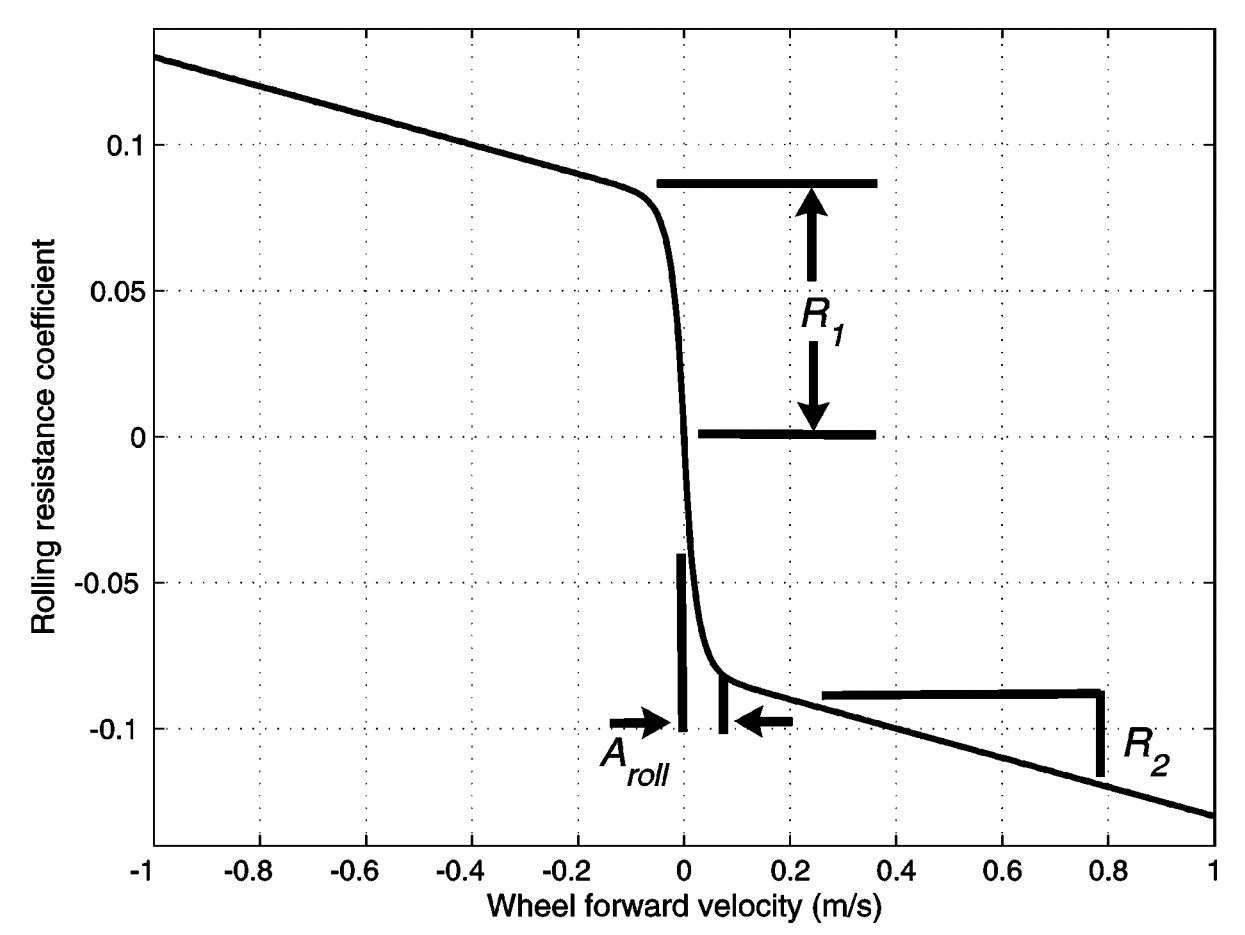
\includegraphics[width = 0.7\textwidth]{imgs/wi_rr}}	
	\caption{Ward-Iagnemma rolling resistance}
	\label{fig:wi_rr}
\end{figure}

This force $F_{rr}$ is then added to $F_{f,lon}$.

Default constants were chosen as in reference paper and showed good stability and robust results. In addition, they can be altered via configuration file. 



\newpage


\subsection{Vehicle models}

Vehicle models are fully configurable with world XML files. 

\subsubsection{Vehicle base class}

Vehicle base incorporates basic functions for every vehicle actor in the scene. It is also responsible for updating state of vehicles.

It has implementation of interaction with world. Derived classes re-implement only work with torques/forces on wheels. 

At the moment, no model takes into account the weight transfer, so weight on wheels is calculated in this base class.

Vehicle base class also provides ground-truth for velocity and position. 
\begin{center}
\[
p_w = \frac{p_{chassis}}{N_w}
\]
\end{center}

\begin{itemize}
	\item Before time step:
	\begin{itemize}
		\item Update wheels position using Box2D
		\item Invoke motor controllers (reimplemented in derived classes)
		\item Evaluate friction of wheels with passed friction model
		\item Apply force to vehicle body using Box2D
	\end{itemize}
	\item Time step - update internal vehicle state variables $q$ and $\dot{q}$
	\item After time step - updates wheels rotation		
\end{itemize}

Center of mass is defined as center of Box2D shape, currently there is no +Z mobility. 
 
\subsubsection{Differential driven}

A differential wheeled robot is a mobile robot whose movement is based on two separately driven wheels placed on either side of the robot body. It can thus change its direction by varying the relative rate of rotation of its wheels and hence does not require an additional steering motion.

\textit{Odometry-based velocity estimation} is implemented via Euler formula (consider revising, it doesn't include side slip):
\[
\omega_{veh} = \frac{\omega_r \cdot R_r - \omega_l \cdot R_r}{y_r - y_l}
\]
\[
\nu_x = \omega_l \cdot R_l + \omega \cdot y_l
\]
\[
\nu_y = 0
\]
Where $\omega_{veh}$ is angular velocity of the robot, $R_i$ - radius of the wheel, $y_i$ is the y position of the wheel, $\omega_i$ is the angular velocity of the wheel. All calculations in the robot's local frame. 

\textit{Nothing more interesting here.}
\subsubsection{Ackermann driven}

Ackermann steering geometry is a geometric arrangement of linkages in the steering of a car or other vehicle designed to solve the problem of wheels on the inside and outside of a turn needing to trace out circles of different radii.

\textit{Ackermann wheels' angles }are computed as following:
\[
\alpha_{outer} = atan(cot(|\alpha| + \frac{w}{2l})
\]
\[
\alpha_{inner} = atan(cot(|\alpha| - \frac{w}{2l})
\]
where $\alpha$ is the desired equivalent steering angle, $w$ is wheels distance and $l$ is wheels base.
Outer and inner wheel are defined by the turn direction.



\textit{Odometry-based velocity estimation} is implemented via Euler formula (consider revising, it doesn't include side slip):
\[
\omega_{veh} = \frac{\omega_{rr} \cdot R_{rr} - \omega_{rl} \cdot R_{rr}}{y_{rr} - y_{rl}}
\]
\[
\nu_x = \omega_{rl} \cdot R_{rl} + \omega \cdot y_{rl}
\]
\[
\nu_y = 0
\]
Where $\omega_{veh}$ is angular velocity of the robot, $R_{ri}$ - radius of the rear wheel, $y_{ri}$ is the y position of the rear wheel, $\omega_{ri}$ is the angular velocity of the rear wheel. All calculations in the robot's local frame. 


\subsubsection{Ackermann-driven with drivetrain}

This type of dynamics has the same geometry as simple Ackermann-driven robots. However, its powertrain is completely different. 

Instead of one "motor" per wheel, this type of dynamics incorporates one "motor" linked to wheels by differentials. 

There are two types of differentials:
\begin{itemize}
	\item Open differntial
	\item Torsen-like locking differential \cite{torsen-whitepaper}
\end{itemize}

Each type of differential can be linked with following configurations: 
\begin{itemize}
	\item Front drive
	\item Rear drive
	\item 4WD
\end{itemize}

Split is customizable between all axes.

As engine plays controller, whose torque output is then fed into differentials. 

For open differential act the following equations:

$$
\tau_{FL} = \tau_{motor} \cdot K_{s,f} \cdot K_{s,frl}
$$

$$
\tau_{FR} = \tau_{motor} \cdot K_{s,f} \cdot (1 - K_{s,frl})
$$

$$
\tau_{RL} = \tau_{motor} \cdot K_{s,r} \cdot K_{s,rrl}
$$

$$
\tau_{RR} = \tau_{motor} \cdot K_{s,r} \cdot (1 - K_{s,frl})
$$


Where $K_{s,f}, K_{s,frl}, K_{s,rrl}$ are split coefficients between axes.

Different things happen for Torsen-like differentials. 
As this type is self-locking, its torque output per wheel depends on wheel's velocity. Here is the function of selecting torque on the next time step based on previous time step velocity. First, introduce the bias ratio - the ratio indicating how much more torque the Torsen can send to the tire with more available traction, than is used by the tire with less traction. This ratio represents the "locking effect" of the differential. By default, it is set to $b = 1.5$

$\omega_1, \omega_2$ and $t_1, t_2$ are the output axles angular velocities and torque splits respectively. $K_s$ is differential split when it is not locked.

$$
\omega_{max} = max(|\omega_1|, |\omega_2|)
$$

$$
\omega_{min} = min(|\omega_1|, |\omega_2|)
$$

$$
\delta_{lock} = \omega_{max} - b \cdot \omega_{min}
$$

$$
\delta_t = 
\begin{cases}
	\delta_{lock} \cdot \omega_{max}, & \mbox{if } \delta_{lock} > 0 \\
	0, & \mbox{if } \delta_{lock} \leq 0
\end{cases}
$$

$$
f_1 = 
\begin{cases}
	K_s \cdot (1 - \delta_t) & \mbox{if } |\omega_1| - |\omega_2| > 0 \\
	K_s \cdot (1 + \delta_t)
\end{cases}
$$
$$
f_2 = 
\begin{cases}
	(1 - K_s) \cdot (1 + \delta_t) & \mbox{if } |\omega_1| - |\omega_2| > 0 \\
	(1 - K_s) \cdot (1 - \delta_t)
\end{cases}
$$

$$
t_1 = \frac{f_1}{f_1 + f_2}
$$

$$
t_2 = \frac{f_2}{f_1 + f_2}
$$

Torque delivery for 2WD is pretty straightforward. There is one input from "motor" and two outputs to wheels, so wheel torques are:

$$
\tau_i = \tau_{motor} \cdot t_i
$$

where $t_i$ is the output of Torsen differential for $i$-th wheel.

With 4WD, torque is first split with Torsen to front and rear parts, each of them is than split independently with another Torsen.

At the moment, there is no model of the engine and thus no feedback of tires torque to engine. 


\subsection{Controllers}

Different vehicles have different controllers. 
At the moment, differential and Ackermann drives have their own controllers. 

Controllers are divided into several types: 
\begin{itemize}
\item Raw forces
\item Twist
\end{itemize}

Ackermann has controller, which controls steering angle and speed. 

Controllers' input and output are described by dynamics' classes that they use. 

\subsubsection{Differential raw controller}

This type of controller has simple response to user's input integrating wheel torque with each simulation frame.

\subsubsection{Differential Twist controller}

Differential twist controller uses PID regulator to control linear and angular speed of the robot. 

Setpoints for $v_r$ and $v_l$ are calculated as following:
$$
v_l = \nu - \frac{\omega}{2} \cdot w
$$
$$
v_r = \nu + \frac{\omega}{2} \cdot w
$$

where $\nu$ is desired linear velocity and $\omega$ is desired angular velocity.


Inverted formula are suitable to get actual velocities from odometry estimates.


Then, velocity of the wheels is controlled with PID regulator.

\subsubsection{Ackermann raw controller}

As a raw differential controller, raw Ackermann controller integrates user input and sets wheel torques and steering wheel angle.

\subsubsection{Ackermann twist controller}

Ackermann twist controller uses PID regulator to control wheel torques responding to angular and linear velocity commands. 
Turn radius and desired steering angle are calculated: 
$$
R = \frac{\nu_s}{\omega_s}
$$
$$
\alpha = atan(\frac{w}{r})
$$

Desired velocities for wheels are computed by rotating desired linear velocity to the steering angle. 
In the same way, actual velocities from "odometry" are computed.

Then, torque of separate wheels is controlled with PID regulators for each wheel.

\subsubsection{Ackermann steering controller}

Ackermann steering controller takes as input linear speed an steering angle. 

Then, it executes Ackermann twist controller to control wheels' torques. 

\subsubsection{Ackermann-drivetrain controllers}

These controllers' steering is identical to Ackermann contollers, however, their torque part is different. 

These controllers' output acts like 'engine' for drivetrain. Instead of separate outputs to wheels, it has one torque output to differentials that will split it to separate wheels. 

\nocite{*}
\bibliographystyle{plain}
\bibliography{bibfile}


\end{document}
